\documentclass[aspectratio=169]{beamer}
\usepackage{will_handley_beamer}
\usepackage{title_page}

% Commands
% --------
% - \arxiv{arxiv number}
% - \arxiv{<number>}            arxiv.org/abs/<number>
% - \oldarxiv{<arxiv number>}   arxiv.org/<number>
% - \doi{<doi>}                 doi.org/<doi>
% - \xkcd{<number>}             xkcd.com/<number>
% - \email{<email>}             <<email>>
% - \tthref{<website>}          <website>
% - \av[dist]{<quantity>}       <quantity>_{dist}
% - \student{<name>}{<detail>}{<photo>}

% A simple command for highlighting key terms
\newcommand{\keyterm}[1]{\textbf{\textcolor{C0}{#1}}}

% Talk details
% ------------
\title{GPU Accelerated Bayesian Inference for Astronomy}
\date{22 October 2025}

\begin{document}

\begin{frame}
    \titlepage
\end{frame}

% --- PEDAGOGICAL FOUNDATION (from sed_2025) ---

% --- SLIDE 2: From Photons to Physics ---
\begin{frame}
    \frametitle{The Goal: From Photons to Physics}
    \framesubtitle{Why astronomical inference is a statistical problem}
    \begin{columns}[T]
        \column{0.49\textwidth}
        \begin{block}{The Data $D$}
            We observe astronomical signals across different wavelengths, time, or frequency. This is our dataset, $D$.
        \end{block}
        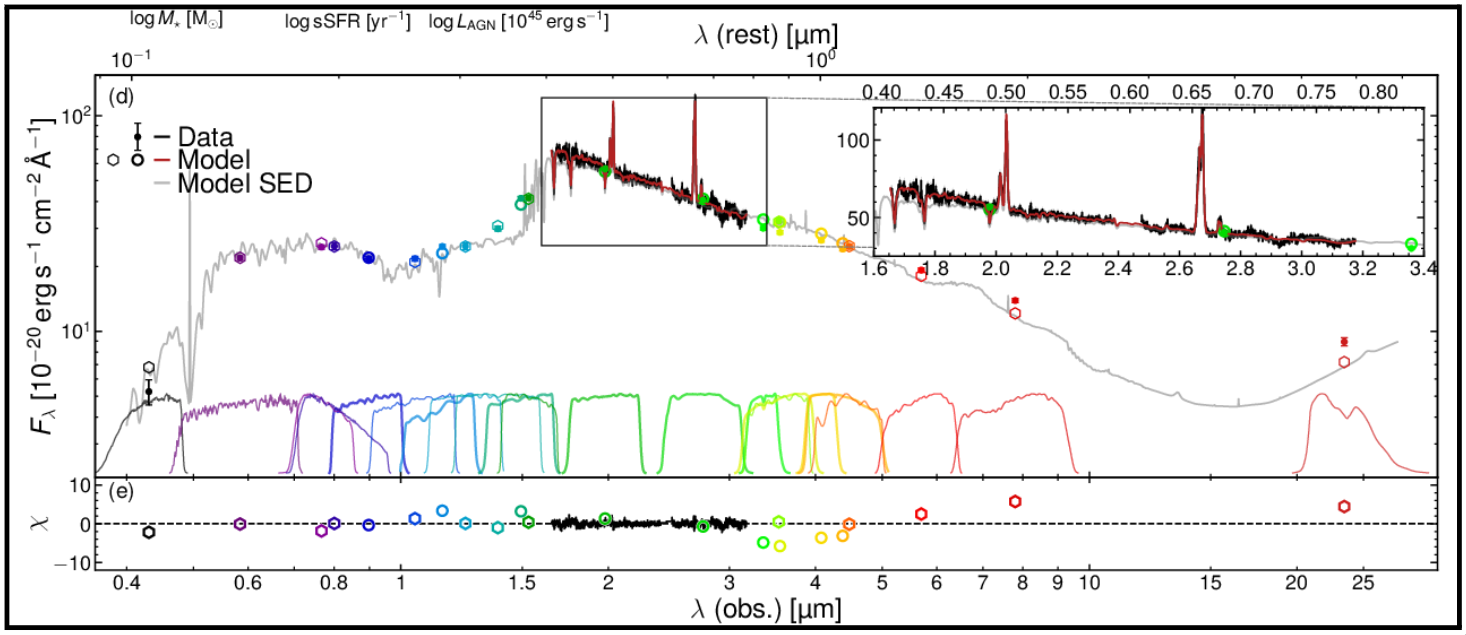
\includegraphics[width=\textwidth]{figures/sed.png}
        \column{0.49\textwidth}
        \begin{block}{The Model $\theta|M$}
            We want to infer the underlying physical properties, our parameters, $\theta$: masses, distances, cosmological parameters, astrophysical properties...
        \end{block}
        \begin{block}{The Challenge}
            The parameter space is often:
            \begin{itemize}
                \item \keyterm{High-dimensional}: Many parameters to fit.
                \item \keyterm{Degenerate}: Different combinations of parameters can produce similar observations.
                \item \keyterm{Multimodal}: Multiple physically plausible explanations.
            \end{itemize}
        \end{block}
    \end{columns}
\end{frame}

% --- SLIDE 3: Statistical Framework ---
\begin{frame}
    \frametitle{The Language of Inference}
    \framesubtitle{How we quantify what we learn from data}
    \begin{columns}
        \column{0.33\textwidth}
            \begin{block}{\C[1]{Prior}\hfill $\C[1]{\pi(\theta)}$}
                What we believe about the parameters \textit{before} we see the data. Our physical assumptions.
            \end{block}
        \vspace{2em}
        \begin{block}{\C[3]{Evidence}\hfill $\C[3]{\mathcal{Z}(D)}$}
            How we update our belief in the model using the data.
        \end{block}
        \column{0.33\textwidth}
\[\underbrace{\C[0]{\mathcal{P}(\theta|D)}}_{\C[0]{\text{Posterior}}} = \frac{\overbrace{\C[2]{\mathcal{L}(D|\theta)}}^{\C[2]{\text{Likelihood}}} \times \overbrace{\C[1]{\pi(\theta)}}^{\C[1]{\text{Prior}}}}{\underbrace{\C[3]{\mathcal{Z}(D)}}_{\C[3]{\text{Evidence}}}}\]
        \column{0.33\textwidth}
            \begin{block}{\C[2]{Likelihood}\hfill $\C[2]{\mathcal{L}(D|\theta)}$}
                How we update our belief in the parameters using the data.
            \end{block}
        \vspace{2em}
        \begin{block}{\C[0]{Posterior}\hfill $\C[0]{\mathcal{P}(\theta|D)}$}
            What we know about the parameters \textit{after} seeing the data. It's our updated state of knowledge.
        \end{block}
    \end{columns}
\end{frame}

% --- SLIDE 4: Chi-squared Maximization ---
\begin{frame}
    \frametitle{The Simplest Approach: Optimization (e.g., $\chi^2$ Minimization)}
    \begin{columns}[T]
        \column{0.5\textwidth}
        \only<1-6>{
        \begin{block}{How it Works: Hill Climbing}
            Imagine the parameter space is a landscape where lower $\chi^2$ (or higher likelihood) is ``downhill''.
            \begin{itemize}
                \item Start somewhere.
                \item Follow the steepest gradient downhill.
                \item Stop when you reach the bottom of a valley.
            \end{itemize}
        \end{block}
        \begin{block}{Advantages}
            \begin{itemize}
                \item \keyterm{Fast} and computationally cheap.
                \item Good for a quick first look.
            \end{itemize}
        \end{block}
        }
        \only<7-10>{
        \begin{block}{Limitations}
            \begin{itemize}
                \item Only gives a single \keyterm{point estimate} (the ``best fit'').
                \item \textbf{No uncertainty quantification!} Where are the error bars?
                \item Can easily get stuck in a \keyterm{local minimum}, missing the true global best fit.
            \end{itemize}
        \end{block}
        \begin{alertblock}{Key Message}
            Optimization is fast but gives an incomplete and potentially misleading picture. Science needs error bars.
        \end{alertblock}
        }
        \column{0.5\textwidth}
        \vspace{-1.8em}
        \begin{center}
            \includegraphics<1>[width=\textwidth,page=1]{figures/himmelblau_gradient_ascent.pdf}%
            \includegraphics<2>[width=\textwidth,page=2]{figures/himmelblau_gradient_ascent.pdf}%
            \includegraphics<3>[width=\textwidth,page=3]{figures/himmelblau_gradient_ascent.pdf}%
            \includegraphics<4>[width=\textwidth,page=4]{figures/himmelblau_gradient_ascent.pdf}%
            \includegraphics<5>[width=\textwidth,page=5]{figures/himmelblau_gradient_ascent.pdf}%
            \includegraphics<6>[width=\textwidth,page=6]{figures/himmelblau_gradient_ascent.pdf}%
            \includegraphics<7>[width=\textwidth,page=7]{figures/himmelblau_gradient_ascent.pdf}%
            \includegraphics<8>[width=\textwidth,page=8]{figures/himmelblau_gradient_ascent.pdf}%
            \includegraphics<9>[width=\textwidth,page=9]{figures/himmelblau_gradient_ascent.pdf}%
            \includegraphics<10>[width=\textwidth,page=10]{figures/himmelblau_gradient_ascent.pdf}%
        \end{center}
    \end{columns}

\end{frame}

% --- SLIDE 5: Why do sampling? ---
\begin{frame}
    \frametitle{Why do sampling?}
    \begin{columns}[T]
        \column{0.5\textwidth}
        \begin{itemize}
            \item The cornerstone of numerical Bayesian inference is working with \textbf{samples}.
            \item Generate a set of representative parameters drawn in proportion to the posterior $\theta\sim\mathcal{P}$.
            \item The magic of marginalisation $\Rightarrow$ perform usual analysis on each sample in turn.
            \item The golden rule is \textbf{stay in samples} until the last moment before computing summary statistics/triangle plots because \[\boxed{f(\:\av{X}\:)\ne \av{\:f(X)\:}}\]
            \item Generally need $\sim\mathcal{O}(12)$ independent samples to compute a value and error bar.
        \end{itemize}
        \column{0.5\textwidth}
        \vspace{-1.8em}
        \begin{center}
            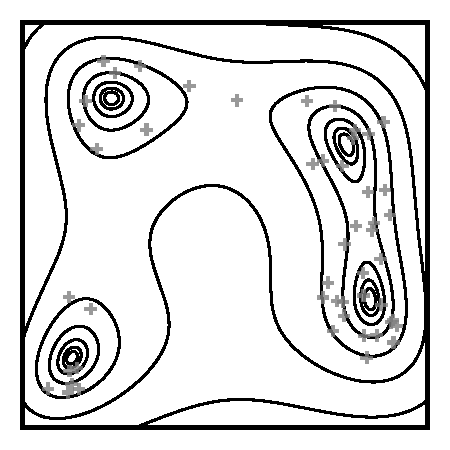
\includegraphics[width=\textwidth]{figures/himmelblau_samples.pdf}
        \end{center}
    \end{columns}
\end{frame}

% --- SLIDE 6: MCMC Sampling ---
\begin{frame}
    \frametitle{The Classic Workhorse: Markov Chain Monte Carlo (MCMC)}
    \begin{columns}[T]
        \column{0.5\textwidth}
        \only<1-5>{
        \begin{block}{How it Works (Metropolis-Hastings)}
            Imagine a ``walker'' exploring the parameter landscape.
            \begin{enumerate}
                \item Take a random step to a new position.
                \item If the new spot is ``higher'' (better likelihood), move there.
                \item If it's ``lower'', maybe move there anyway (with probability proportional to how much lower it is).
                \item Repeat millions of times. The path the walker takes traces the posterior distribution.
            \end{enumerate}
        \end{block}
        }
        \only<6-9>{
            \vspace{-1em}
        \begin{block}{Advantages \& Limitations}
            \begin{itemize}
                \item Explores the full posterior and gives uncertainties.
                \item \textcolor{red}{Limitation:} The walker can be inefficient. It can get ``stuck'' in a local high-likelihood region and fail to find other, separate modes.
                \item \textcolor{red}{Limitation:} Can be slow to explore highly correlated (``banana-shaped'') posteriors.
            \end{itemize}
        \end{block}
        \begin{alertblock}{Key Message}
            MCMC is a foundational sampling method, but its simple ``random walk'' can be inefficient in the complex parameter spaces of astronomical inference.
        \end{alertblock}
        }
        \column{0.5\textwidth}
        \vspace{-1.8em}
        \begin{center}
            \includegraphics<1>[page=1]{figures/himmelblau_mcmc.pdf}%
            \includegraphics<2>[page=2]{figures/himmelblau_mcmc.pdf}%
            \includegraphics<3>[page=3]{figures/himmelblau_mcmc.pdf}%
            \includegraphics<4>[page=4]{figures/himmelblau_mcmc.pdf}%
            \includegraphics<5>[page=5]{figures/himmelblau_mcmc.pdf}%
            \includegraphics<6>[page=6]{figures/himmelblau_mcmc.pdf}%
            \includegraphics<7>[page=7]{figures/himmelblau_mcmc.pdf}%
            \includegraphics<8>[page=8]{figures/himmelblau_mcmc.pdf}%
            \includegraphics<9>[page=9]{figures/himmelblau_mcmc.pdf}%
        \end{center}
    \end{columns}
\end{frame}

% --- SLIDE 7: Hamiltonian Monte Carlo (HMC) ---
\begin{frame}
    \frametitle{Gradient-Guided Sampling: Hamiltonian Monte Carlo (HMC)}
    \begin{columns}[T]
        \column{0.5\textwidth}
        \only<1-5>{
        \begin{block}{How it Works}
            Uses gradients to guide exploration more efficiently than random walks.
            \begin{enumerate}
                \item Treat parameters as ``particles'' with position and momentum.
                \item Use gradient of log-likelihood as ``force'' to guide movement.
                \item Propose coherent moves along gradient directions.
                \item Accept/reject using Metropolis criterion.
            \end{enumerate}
        \end{block}
        }
        \only<6-9>{
        \begin{block}{Advantages \& Requirements}
            \begin{itemize}
                \item Much more efficient than random walk for smooth posteriors.
                \item Requires gradients of the likelihood function.
                \item Can traverse parameter space much faster.
                \item Less likely to get stuck in local regions.
            \end{itemize}
        \end{block}
        \begin{alertblock}{Key Message}
            HMC leverages gradient information for efficient sampling, but requires differentiable models.
        \end{alertblock}
        }
        \column{0.5\textwidth}
        \vspace{-1.8em}
        \begin{center}
            \includegraphics<1>[width=\textwidth,page=1]{figures/himmelblau_hmc.pdf}%
            \includegraphics<2>[width=\textwidth,page=2]{figures/himmelblau_hmc.pdf}%
            \includegraphics<3>[width=\textwidth,page=3]{figures/himmelblau_hmc.pdf}%
            \includegraphics<4>[width=\textwidth,page=4]{figures/himmelblau_hmc.pdf}%
            \includegraphics<5>[width=\textwidth,page=5]{figures/himmelblau_hmc.pdf}%
            \includegraphics<6>[width=\textwidth,page=6]{figures/himmelblau_hmc.pdf}%
            \includegraphics<7>[width=\textwidth,page=7]{figures/himmelblau_hmc.pdf}%
            \includegraphics<8>[width=\textwidth,page=8]{figures/himmelblau_hmc.pdf}%
            \includegraphics<9>[width=\textwidth,page=9]{figures/himmelblau_hmc.pdf}%
        \end{center}
    \end{columns}
\end{frame}

% --- SLIDE 8: Ensemble Sampling (emcee) ---
\begin{frame}
    \frametitle{A Better Way: Ensemble Sampling (e.g., \texttt{emcee})}
    \begin{columns}[T]
        \column{0.5\textwidth}
        \only<1-5>{
        \begin{block}{How it Works}
            Instead of one walker, we use an \keyterm{ensemble} of hundreds of walkers.
            \begin{itemize}
                \item The walkers don't move completely randomly.
                \item They propose new steps based on the positions of \textit{other} walkers in the ensemble.
                \item This allows the whole group to learn about the shape of the posterior (e.g., its correlations) and explore it more efficiently.
            \end{itemize}
        \end{block}
        }
        \only<6-9>{
        \vspace{-1em}
        \begin{block}{Advantages}
            \begin{itemize}
                \item Much better at exploring correlated, ``banana-shaped'' parameter spaces.
                \item More efficient ``mixing'' than a single chain.
                \item Easy to parallelize (one walker per CPU).
            \end{itemize}
        \end{block}
        \begin{block}{Limitation}
            \begin{itemize}
                \item Ensemble can still get trapped in one mode if other modes are very far away.
            \end{itemize}
        \end{block}
        \begin{alertblock}{Key Message}
            Ensemble samplers like \texttt{emcee} are a major improvement for many problems, especially those with parameter degeneracies.
        \end{alertblock}
        }
        \column{0.5\textwidth}
        \vspace{-1.8em}
        \begin{center}
            \includegraphics<1>[width=\textwidth,page=1]{figures/himmelblau_emcee.pdf}%
            \includegraphics<2>[width=\textwidth,page=2]{figures/himmelblau_emcee.pdf}%
            \includegraphics<3>[width=\textwidth,page=3]{figures/himmelblau_emcee.pdf}%
            \includegraphics<4>[width=\textwidth,page=4]{figures/himmelblau_emcee.pdf}%
            \includegraphics<5>[width=\textwidth,page=5]{figures/himmelblau_emcee.pdf}%
            \includegraphics<6>[width=\textwidth,page=6]{figures/himmelblau_emcee.pdf}%
            \includegraphics<7>[width=\textwidth,page=7]{figures/himmelblau_emcee.pdf}%
            \includegraphics<8>[width=\textwidth,page=8]{figures/himmelblau_emcee.pdf}%
            \includegraphics<9>[width=\textwidth,page=9]{figures/himmelblau_emcee.pdf}%
        \end{center}
    \end{columns}
\end{frame}

% --- SLIDE 9: Why Evidence Calculation Matters ---
\begin{frame}
    \frametitle{The Missing Piece: Why Evidence Calculation Matters}
    \framesubtitle{And why it's so hard to compute}
    \begin{columns}[T]
        \column{0.49\textwidth}
        \begin{block}{Why Evidence is Important}
            \begin{itemize}
                \item \textbf{Model Comparison}: Bayes model theorem:
            \[\mathcal{P}(M|D) \propto \mathcal{Z}(D|M) \mathcal{P}(M)\]
            For astronomy: Which physical model best explains the observations?
        \item  \textbf{Occam's Razor}: Automatic complexity penalty
            \[\log \mathcal{Z} = \langle \log \mathcal{L} \rangle_{\mathcal{P}} - \mathcal{D}_{\text{KL}}(\mathcal{P}||\pi)\]
        \item \textbf{Bayesian Model Averaging}: Weighted model combinations
            \end{itemize}
        \end{block}
        \column{0.49\textwidth}
        \begin{block}{Why Evidence is Hard}
            \begin{itemize}
                \item The high-dimensional evidence integral:
            \[\mathcal{Z} = \int \mathcal{L}(\theta) \pi(\theta) d\theta\]
            \[\left(\text{from Bayes theorem}:\mathcal{P}(\theta|D) = \frac{\mathcal{L}(\theta) \pi(\theta)}{\mathcal{Z}}\right)\]
            \pause
        \item The difficulty is \textbf{not} that most of parameter space has $\mathcal{L} \approx 0$...
            \pause
        \item The difficulty is that we can't estimate \textbf{volume} $d\theta$ in high dimensions!
            \end{itemize}
        \end{block}
    \end{columns}
\end{frame}

% --- SLIDE 10: Nested Sampling ---
\begin{frame}
    \frametitle{The State of the Art: Nested Sampling (e.g., \texttt{dynesty})}
    \begin{columns}[T]
        \column{0.5\textwidth}
        \only<1-4>{
        \begin{block}{A Radically Different Approach}
            Instead of random walking, nested sampling attacks the problem from the outside-in.
            \begin{enumerate}
                \item Start with a set of ``live points'' scattered across the entire \keyterm{prior}.
                \item At each step: find the point with the \textit{worst} likelihood and discard it.
                \item Replace it with a new point drawn from the prior, but with a likelihood \textit{better} than the point you just discarded.
                \item This forces the set of live points to continuously ``shrink'' into regions of higher and higher likelihood.
            \end{enumerate}
        \end{block}
        }
        \only<5-8>{
        \begin{block}{Key Advantages}
            \begin{itemize}
                \item Naturally handles \keyterm{multimodality}. The shrinking cloud of points will find and explore all modes simultaneously.
                \item It calculates the \keyterm{Bayesian Evidence} ($\C[3]{\mathcal{Z}}$) as a primary output. This is essential for model comparison!
            \end{itemize}
        \end{block}
        \begin{alertblock}{Key Message}
            Nested sampling excels at exploring complex, multimodal posteriors and is the go-to method for Bayesian model comparison.
        \end{alertblock}
        }
        \column{0.5\textwidth}
        \vspace{-1.8em}
        \begin{center}
            \includegraphics<1>[width=\textwidth,page=1]{figures/himmelblau_ns.pdf}%
            \includegraphics<2>[width=\textwidth,page=2]{figures/himmelblau_ns.pdf}%
            \includegraphics<3>[width=\textwidth,page=3]{figures/himmelblau_ns.pdf}%
            \includegraphics<4>[width=\textwidth,page=4]{figures/himmelblau_ns.pdf}%
            \includegraphics<5>[width=\textwidth,page=5]{figures/himmelblau_ns.pdf}%
            \includegraphics<6>[width=\textwidth,page=6]{figures/himmelblau_ns.pdf}%
            \includegraphics<7>[width=\textwidth,page=7]{figures/himmelblau_ns.pdf}%
            \includegraphics<8>[width=\textwidth,page=8]{figures/himmelblau_ns.pdf}%
        \end{center}
    \end{columns}
\end{frame}

% --- SLIDE 11: How Nested Sampling Estimates Volumes ---
\begin{frame}
    \frametitle{How Nested Sampling Estimates Volumes: The Counting Trick}
    \begin{columns}[T]
        \column{0.5\textwidth}
        \begin{block}{Volume Contraction}
            At each step, the volume contracts predictably:
            \[V_{i+1} = V_i \times \frac{n_{\text{inside}}}{n_{\text{total}}}\]
            indep.\ of dimensionality, geometry or topology
        \end{block}

        \begin{columns}[T]
            \column{0.45\textwidth}
            \begin{block}{Evidence}
                The evidence is computed as:
                \[\mathcal{Z} = \sum \mathcal{L}_i \Delta V_i\]
            \end{block}

            \column{0.45\textwidth}
            \begin{block}{Posterior}
                Each sample gets importance weight:
                \[w_i = \mathcal{L}_i \times \Delta V_i\]
            \end{block}
        \end{columns}
        \column{0.5\textwidth}
        \vspace{-1.8em}
        \begin{center}
            \includegraphics<1>[width=\textwidth,page=1]{figures/himmelblau_ns_counting_trick.pdf}
            \includegraphics<2>[width=\textwidth,page=2]{figures/himmelblau_ns_counting_trick.pdf}
            \includegraphics<3>[width=\textwidth,page=3]{figures/himmelblau_ns_counting_trick.pdf}
            \includegraphics<4>[width=\textwidth,page=4]{figures/himmelblau_ns_counting_trick.pdf}
            \includegraphics<5>[width=\textwidth,page=5]{figures/himmelblau_ns_counting_trick.pdf}
            \includegraphics<6>[width=\textwidth,page=6]{figures/himmelblau_ns_counting_trick.pdf}
            \includegraphics<7>[width=\textwidth,page=7]{figures/himmelblau_ns_counting_trick.pdf}
            \includegraphics<8>[width=\textwidth,page=8]{figures/himmelblau_ns_counting_trick.pdf}
            \includegraphics<9>[width=\textwidth,page=9]{figures/himmelblau_ns_counting_trick.pdf}
        \end{center}
        \begin{center}
            \only<1>{\textbf{200 live points}}
            \only<2>{\textbf{Mark for deletion}}
            \only<3>{\textbf{Delete points}}
            \only<4>{\textbf{Repopulate}}
            \only<5>{\textbf{Next iteration}}
            \only<6>{\textbf{Delete again}}
            \only<7>{\textbf{Repopulate again}}
            \only<8>{\textbf{Complete sampling}}
            \only<9>{\textbf{Posterior reweighting}}
        \end{center}
    \end{columns}
\end{frame}

% --- SLIDE 12: Practical Guidance for Nested Sampling ---
\begin{frame}
    \frametitle{Practical Guidance: How to Use Nested Sampling}
    \framesubtitle{Understanding resolution and reliability parameters}
    \vspace{-1em}
    \begin{columns}[T]
        \column{0.49\textwidth}
        \begin{block}{Rejection Samplers}
            \begin{itemize}
                \item e.g. \texttt{MultiNest}, \texttt{UltraNest}, \texttt{nessai}
                \item Construct bounding regions, reject invalid points
                \item Efficient in low dimensions ($d \lesssim 10$)
                \item Exponentially inefficient in high dimensions
            \end{itemize}
        \end{block}
        \column{0.49\textwidth}
        \begin{block}{Chain-based Samplers}
            \begin{itemize}
                \item e.g. \texttt{PolyChord}, \texttt{dynesty}, \texttt{blackjax}
                \item Run Markov chains from live points
                \item Linear $\sim\mathcal{O}(d)$ scaling penalty
                \item Better for high-dimensional problems
            \end{itemize}
        \end{block}
    \end{columns}
    \vspace{5pt}
    \begin{alertblock}{Key Parameters}
        \begin{itemize}
            \item \textbf{Resolution parameter} $n_{\text{live}}$: Improves results as $\sim\mathcal{O}(n_{\text{live}}^{-1/2})$
            \item \textbf{Reliability parameters}: Don't improve results if set arbitrarily high, but introduce systematic errors if set too low
                \begin{itemize}
                    \item \texttt{MultiNest} efficiency \texttt{eff}, \texttt{PolyChord} chain length \texttt{n\_repeats}, \texttt{dynesty} \texttt{slices}
                \end{itemize}
        \end{itemize}
    \end{alertblock}
\end{frame}

% --- SLIDE 13: Choosing Your Tool ---
\begin{frame}
    \frametitle{Choosing Your Tool: A Summary}
    \framesubtitle{No single best method, only the right tool for the job}
    \begin{center}
        \begin{tabular}{|l|c|c|c|c|}
            \hline
            \textbf{Method} & \textbf{Speed} & \textbf{Uncertainties?} & \textbf{Handles Multimodality?} & \textbf{Evidence?} \\
            \hline
            \textbf{Optimization} ($\chi^2$) & \textcolor{green!50!black}{Very Fast} & \textcolor{red}{No} & \textcolor{red}{No} & \textcolor{red}{No} \\
            \hline
            \textbf{MCMC} (\texttt{pymc} etc) & \textcolor{orange}{Medium} & \textcolor{green!50!black}{Yes} & \textcolor{orange}{Poorly} & \textcolor{red}{No} \\
            \hline
            \textbf{HMC} (\texttt{stan}, \texttt{numpyro}) & \textcolor{orange}{Medium} & \textcolor{green!50!black}{Yes} & \textcolor{orange}{Okay} & \textcolor{red}{No*} \\
            \hline
            \textbf{Ensemble} (\texttt{emcee}) & \textcolor{orange}{Medium} & \textcolor{green!50!black}{Yes} & \textcolor{orange}{Okay} & \textcolor{red}{No} \\
            \hline
            \textbf{Nested} (\texttt{dynesty}) & \textcolor{red}{Slower} & \textcolor{green!50!black}{Yes} & \textcolor{green!50!black}{Excellently} & \textcolor{green!50!black}{Yes!} \\
            \hline
        \end{tabular}
    \end{center}
    \begin{block}{Practical Guidance}
        \begin{itemize}
            \item \textbf{Quick exploration / Sanity check?} $\rightarrow$ Use Optimization.
            \item \textbf{Simple, well-behaved posterior?} $\rightarrow$ \texttt{emcee} is a great choice.
            \item \textbf{Smooth, differentiable posterior?} $\rightarrow$ HMC can be very efficient.
            \item \textbf{Complex, possibly multimodal posterior?} $\rightarrow$ Use \texttt{dynesty}.
            \item \textbf{Need to compare different physical models?} $\rightarrow$ You \textit{must} use Nested Sampling.
        \end{itemize}
    \end{block}
\end{frame}

% --- GPU APPLICATIONS (from caltech_2025) ---

% --- SLIDE 14: GPU Computing ---
\begin{frame}
    \frametitle{GPU Computing: Beyond Machine Learning}
    \begin{columns}
        \column{0.48\textwidth}
        \begin{block}{GPU vs CPU for Scientific Computing}
            \begin{itemize}
                \item \textbf{CPU}: Few powerful cores (10s), complex control.
                \item \textbf{GPU}: Many simple cores (1000s), simple control.
                \item \textbf{Memory bandwidth}: GPU ~10× faster than CPU.
                \item \textbf{Perfect for}: Independent parallel tasks.
                \item \textbf{Scientific algorithms}: MCMC chains, likelihood evaluations, simulations.
            \end{itemize}
        \end{block}
        \column{0.48\textwidth}
        \begin{block}{HPC Landscape Evolution}
            \begin{itemize}
                \item HPC transitioning to GPU-based architectures.
                \item ML adoption accelerating hardware development.
                \item Legacy CPU codes require modernization.
            \end{itemize}
        \end{block}
        \begin{block}{Key Point}
            \begin{center}
                \textbf{GPU $\neq$ Machine Learning}\\
                GPUs accelerate any parallel algorithm
            \end{center}
        \end{block}
    \end{columns}
\end{frame}

% --- SLIDE 15: Modern Languages: Two Independent Capabilities ---
\begin{frame}
    \frametitle{Modern Languages: Two Independent Capabilities}
    \begin{center}
        \textbf{Differentiable programming languages}: JAX, PyTorch, TensorFlow, Julia, Stan, \ldots
    \end{center}
    \vspace{-5pt}
    \begin{columns}
        \column{0.48\textwidth}
        \begin{block}{Capability 1: Free Gradients}
            \begin{itemize}
                \item \textbf{Automatic differentiation}: $\nabla_\theta \log \mathcal{L}(\theta)$.
                \item Enables gradient-based MCMC (HMC, NUTS).
                \item Essential for modern optimization.
            \end{itemize}
        \end{block}
        \begin{block}{Traditional Physics Benefits}
            \begin{itemize}
                \item \textbf{Nested sampling}: Massive parallelization.
                \item \textbf{21cm signals}: Vectorized across frequency/time/angle.
                \item \textbf{N-body sims}: GPU acceleration.
            \end{itemize}
        \end{block}
        \column{0.48\textwidth}
        \begin{block}{Capability 2: GPU Parallelization}
            \begin{itemize}
                \item \textbf{Vectorization across ensembles}.
                \item Run 1000s of parallel chains/particles.
                \item Evaluate likelihoods simultaneously.
            \end{itemize}
        \end{block}
        \begin{block}{Key Insight: Often Confused}
            \begin{center}
                \textbf{These are completely independent.}\\
                \textbf{People mistake one for the other.}\\
                You can use gradients on CPU.\\
                You can GPU parallelize without gradients.\\
                \textbf{They serve different purposes.}
            \end{center}
        \end{block}
    \end{columns}
\end{frame}

% --- BRIDGE SLIDE: Where do GPUs help in inference? ---
\begin{frame}
    \frametitle{Where do GPUs help in Bayesian Inference?}
    \framesubtitle{Mapping algorithmic structure to parallel hardware}
    \begin{columns}
        \column{0.48\textwidth}
        \begin{block}{Parallel Structures}
            \begin{itemize}
                \item \textbf{Parallel chains/particles/live points}
                    \begin{itemize}
                        \item MCMC ensembles (\texttt{emcee})
                        \item SMC particle swarms
                        \item Nested sampling live points
                    \end{itemize}
                \item \textbf{Vectorize likelihoods across batches}
                    \begin{itemize}
                        \item Evaluate hundreds of parameter sets simultaneously
                        \item Perfect for GPU SIMD architecture
                    \end{itemize}
            \end{itemize}
        \end{block}
        \column{0.48\textwidth}
        \begin{block}{GPU Best Practices}
            \begin{itemize}
                \item \textbf{JIT compilation}
                    \begin{itemize}
                        \item Compile once, run many times
                        \item Avoid host-device transfers
                    \end{itemize}
                \item \textbf{When gradients matter}
                    \begin{itemize}
                        \item Essential: HMC/NUTS
                        \item Not required: NS/ensemble/MCMC
                    \end{itemize}
                \item \textbf{Device RNG}
                    \begin{itemize}
                        \item Reproducibility requires careful seeding
                    \end{itemize}
            \end{itemize}
        \end{block}
    \end{columns}
\end{frame}

% --- SLIDE 17: BlackJAX: GPU Native Sampling ---
\begin{frame}
    \frametitle{BlackJAX: GPU Native Sampling}
    \framesubtitle{A unified framework for GPU-accelerated inference}
    \student{david_yallup}{David Yallup}{Postdoc}
    \begin{columns}
        \column{0.55\textwidth}
        \begin{block}{The Challenge}
            \begin{itemize}
                \item Sampling traditionally CPU-bound
                \item Different algorithms, same GPU challenge
                \item Need unified GPU-native framework
            \end{itemize}
        \end{block}
        \begin{block}{BlackJAX Solution}
            \begin{itemize}
                \item Full JAX ecosystem integration
                \item All core algorithms GPU-accelerated:
                    \begin{itemize}
                        \item Optimization (gradient descent)
                        \item MCMC (Metropolis-Hastings)
                        \item HMC/NUTS (gradient-guided)
                        \item SMC (particle methods)
                    \end{itemize}
                \item Coming soon (PRs in progress):
                    \begin{itemize}
                        \item Ensemble (emcee) \tthref{github.com/blackjax-devs/blackjax/pull/797}
                        \item Nested sampling \tthref{github.com/blackjax-devs/blackjax/pull/755}
                    \end{itemize}
            \end{itemize}
        \end{block}
        \column{0.43\textwidth}
        \begin{block}{Framework Design}
            \begin{itemize}
                \item Like \texttt{numpy}/\texttt{scipy}
                \item Not like \texttt{cobaya}/\texttt{cosmosis}
                \item Composable building blocks
                \item Maximum flexibility
            \end{itemize}
        \end{block}
        \vspace{10pt}
        \begin{center}
            \includegraphics[width=\textwidth,page=8]{figures/himmelblau_ns.pdf}
        \end{center}
    \end{columns}
\end{frame}

% --- SLIDE 18: Case Study 1: CMB and Cosmic Shear ---
\begin{frame}
    \frametitle{Recent GPU-Accelerated Applications}
    \framesubtitle{Case study 1/4: CMB and Cosmic Shear \arxiv{2509.13307}}
    \student{toby_lovick}{Toby Lovick}{PhD}
    \begin{columns}
        \column{0.48\textwidth}
        \begin{itemize}
            \item \textbf{CMB (6 params)}: 300× speedup vs CPU PolyChord
            \item \textbf{Cosmic Shear (37 params)}: Days vs months ($>$1000× vs CPU; 10× vs GPU NUTS)
            \item \textbf{Method}: JAX neural emulators + GPU NS
            \item \textbf{Evidence}: Direct calculation with error bars
            \item \textbf{Models}: $\Lambda$CDM vs $w_0w_a$ comparison
            \item \textbf{Impact}: NS competitive with MCMC+evidence methods
        \end{itemize}
        \column{0.48\textwidth}
        \includegraphics<1>[width=\textwidth]{figures/cmbscaling.pdf}%
        \vspace{5pt}
        \includegraphics<2>[width=\textwidth]{figures/jaxSHEARfull.png}
    \end{columns}
\end{frame}

% --- SLIDE 19: Case Study 2: Bayesian Anomaly Detection for SNe ---
\begin{frame}
    \frametitle{Recent GPU-Accelerated Applications}
    \framesubtitle{Case study 2/4: Bayesian Anomaly Detection for Type Ia Supernovae \arxiv{2509.13394}}
    \student{sam_leeney}{Sam Leeney}{PhD}
    \begin{columns}
        \column{0.48\textwidth}
        \begin{itemize}
            \item \textbf{Problem}: Manual photometric rejection not scalable for LSST
            \item \textbf{Solution}: Bayesian anomaly detection integrated into SALT3 fitting
            \item \textbf{Method}: Model contamination probability per measurement
            \item \textbf{Result}: Automatic outlier/corrupted band rejection
            \item \textbf{Finding}: Contaminants systematically brighter/bluer
            \item \textbf{Impact}: Essential for unbiased cosmology at scale
        \end{itemize}
        \column{0.48\textwidth}
        \vspace{10pt}
        \includegraphics<1>[width=\textwidth]{figures/2509.13394_19ekb_light_curves_all_paper.png}%
        \includegraphics<2>[width=\textwidth]{figures/2509.13394_recreated_contamination_plot.png}
    \end{columns}
\end{frame}

% --- SLIDE 20: Case Study 3: Dark Energy vs Systematics ---
\begin{frame}
    \frametitle{Recent GPU-Accelerated Applications}
    \framesubtitle{Case study 3/4: Dark Energy vs Supernova Systematics \arxiv{2509.13220}}
    \student{adam_ormondroyd}{Adam Ormondroyd}{PhD}
    \begin{columns}
        \column{0.65\textwidth}
        \begin{itemize}
            \item \textbf{Question}: DESI+DES $w_0w_a$ preference - new physics or systematics?
            \item \textbf{Method}: Bayesian model comparison
            \item \textbf{Models}: Dynamic DE vs redshift-dependent SN bias
            \item \textbf{Result}: Systematics fit equally well with lower complexity
            \item \textbf{Evidence}: Favors systematic explanation
            \item \textbf{Lesson}: Test mundane before claiming exotic
        \end{itemize}
        \column{0.35\textwidth}
        \vspace{10pt}
        \includegraphics<1>[width=\textwidth]{figures/2509.13220_desidr2_des5yoffset_20_wa.pdf}%
        \includegraphics<2>[width=\textwidth]{figures/2509.13220_des5yoffset_20_wa.pdf}
    \end{columns}
\end{frame}

% --- SLIDE 21: Case Study 4: Gravitational Waves ---
\begin{frame}
    \frametitle{Recent GPU-Accelerated Applications}
    \framesubtitle{Case study 4/4: Gravitational Wave Inference \arxiv{2509.04336}}
    \student{metha_prathaban}{Metha Prathaban}{PhD}
    \begin{columns}
        \column{0.48\textwidth}
        \begin{itemize}
            \item \textbf{Goal}: GPU-accelerate bilby's acceptance-walk NS
            \item \textbf{Implementation}: Faithful port to blackjax-ns
            \item \textbf{Performance}: 20-40× speedup for BBH
            \item \textbf{Validation}: Identical posteriors/evidences
            \item \textbf{Hardware}: Single GPU vs CPU clusters
            \item \textbf{Impact}: Clean baseline for future methods
        \end{itemize}
        \column{0.48\textwidth}
        \includegraphics<1>[width=\textwidth]{figures/2509.04336_8s_corner_comparison.pdf}%
        \includegraphics<2>[width=\textwidth]{figures/2509.04336_walltime_speedup.pdf}
    \end{columns}
\end{frame}

% --- SLIDE 22: Getting Started with BlackJAX ---
\begin{frame}[fragile]
    \frametitle{Getting Started with BlackJAX}
    \framesubtitle{Practical steps to GPU-accelerated inference}

    \begin{columns}
        \column{0.48\textwidth}
        \begin{block}{Installation}
            \small
            \texttt{pip install git+https://github.com/\\
            \hspace*{2em}handley-lab/blackjax}
        \end{block}

        \begin{block}{Resources}
            \small
            \begin{itemize}
                \item \textbf{Nested Sampling Book}: \\
                    \tthref{handley-lab.co.uk/nested-sampling-book}
                \item \textbf{Workshop \& Tutorials}: \\
                    \github{handley-lab/workshop}
                \item \textbf{BlackJAX NS PR}: \\
                    \github{blackjax-devs/blackjax} \#755
            \end{itemize}
        \end{block}

        \column{0.48\textwidth}
        \begin{block}{Minimal Example}
            \tiny
            \begin{verbatim}
import jax
import blackjax

# Define model
logL = lambda x: -0.5 * jnp.sum(x**2)
prior = lambda key: jax.random.normal(key, (5,))

# Initialize nested sampling
ns = blackjax.ns(logL, prior, n_live=500)

# Run on GPU
key = jax.random.PRNGKey(0)
state = ns.init(key)
results = ns.run(state, max_samples=5000)
            \end{verbatim}
        \end{block}

        \begin{alertblock}{Key Points}
            \tiny
            \begin{itemize}
                \item Use \texttt{jax.jit} to compile likelihoods
                \item \texttt{vmap} for batch operations
                \item Keep data on device (avoid CPU/GPU transfers)
            \end{itemize}
        \end{alertblock}
    \end{columns}
\end{frame}

% --- SLIDE 23: The Future: AI in Scientific Code Development ---
\begin{frame}[fragile]
    \frametitle{The Future: AI in Scientific Code Development}
    \student{claude}{Claude Code}{AI Assistant}
    \vspace{-1em}
    \begin{columns}[T]
        \column{0.49\textwidth}
        \begin{block}{The Real AI Revolution: LLMs}
            The biggest impact of AI will not be in analyzing data, but in helping us write the code to do it.
            \begin{itemize}
                \item \textbf{Automated code translation}: LLMs can help port legacy Fortran/C++ models to modern, GPU-friendly \& differentiable frameworks like JAX or PyTorch.
            \end{itemize}
        \end{block}
        \column{0.49\textwidth}
        \begin{block}{The 80/20 Rule of Scientific Work}
            \begin{itemize}
                \item \textbf{80\% ``boring'' tasks}: Writing code, debugging, drafting \& reviewing papers, munging data, organising meetings...
                \item \textbf{20\% ``hard thinking''}: The actual scientific insight.
            \end{itemize}
            AI's biggest immediate impact is automating and accelerating the 80\%, freeing up human time for the 20\%.
        \end{block}
    \end{columns}
    \vspace{-0.5em}
    \begin{exampleblock}{Concrete Example: Porting Fortran Likelihood to JAX}
        \small
        \begin{columns}[T]
            \column{0.48\textwidth}
            \textbf{Before (Fortran/Python):}
            \tiny
            \begin{verbatim}
# Serial loop over data
chi2 = 0.0
for i in range(len(data)):
    model = compute_model(params, x[i])
    chi2 += ((data[i] - model) / err[i])**2
logL = -0.5 * chi2
            \end{verbatim}
            \column{0.48\textwidth}
            \textbf{After (JAX):}
            \tiny
            \begin{verbatim}
# Vectorized, JIT-compiled, GPU-ready
@jax.jit
def logL(params):
    model = jax.vmap(compute_model, (None, 0))(params, x)
    chi2 = jnp.sum(((data - model) / err)**2)
    return -0.5 * chi2
# Result: 100x speedup + GPU acceleration
            \end{verbatim}
        \end{columns}
    \end{exampleblock}
    \begin{alertblock}{Key Message}
        AI is not just a tool for analysis; it's about to fundamentally change how we develop, optimize, and deploy our science
    \end{alertblock}
\end{frame}

% --- SLIDE 24: Conclusions ---
\begin{frame}
    \frametitle{Conclusions}
    \framesubtitle{\tthref{github.com/handley-lab/group}}
        \begin{enumerate}
            \item \textbf{Statistical Foundations Matter}
                \begin{itemize}
                    \item From optimization to sampling to model comparison
                    \item Nested sampling uniquely computes evidence
                \end{itemize}
            \item \textbf{GPU $\neq$ Machine Learning: Two Independent Capabilities}
                \begin{itemize}
                    \item GPUs accelerate any parallel algorithm.
                    \item Automatic differentiation + massive parallelization.
                    \item Often confused, serve different purposes.
                \end{itemize}
            \item \textbf{Classical Algorithms on GPU Competitive with ML State of the Art}
                \begin{itemize}
                    \item Traditional physics methods + GPU = superior performance.
                    \item 300× speedup for CMB, 20-40× for gravitational waves
                \end{itemize}
            \item \textbf{AI Accelerates Development as well as Computation}
                \begin{itemize}
                    \item LLMs solve the GPU porting challenge at scale.
                    \item 10× development speedup enables widespread adoption.
                \end{itemize}
        \end{enumerate}
        \vfill
        \begin{alertblock}{Get Started with GPU-Accelerated Sampling}
            \centering
            \Large
            \tthref{handley-lab.co.uk/nested-sampling-book}
        \end{alertblock}
    \tikz[overlay,remember picture]
        \node[anchor=north east] (A) at ($(current page.north east)+(0,0)$) {
        
\includegraphics[width=0.06\textheight]{people/adam_ormondroyd.jpg}%
        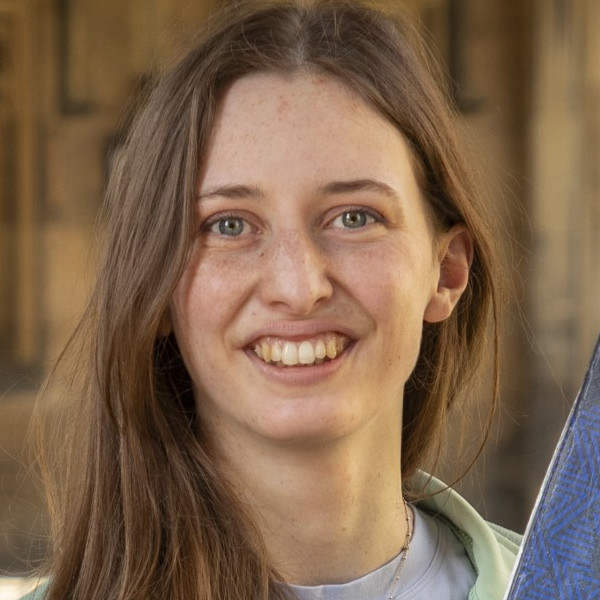
\includegraphics[width=0.06\textheight]{people/charlotte_priestley.jpg}%
        
\includegraphics[width=0.06\textheight]{people/claude.jpg}%
        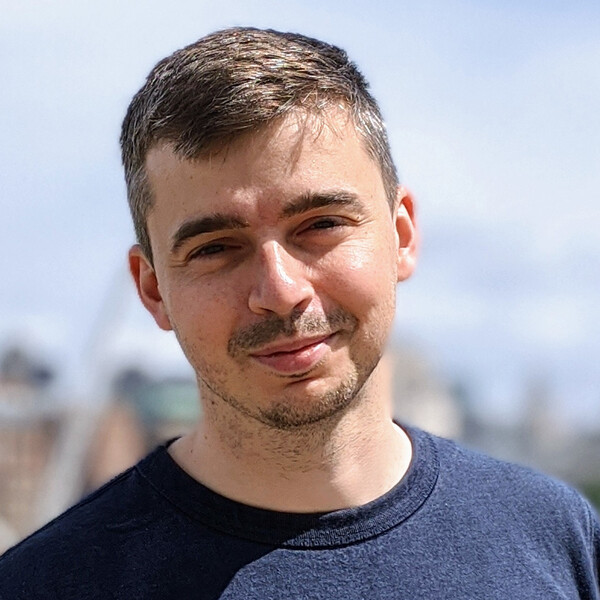
\includegraphics[width=0.06\textheight]{people/david_yallup.jpg}%
        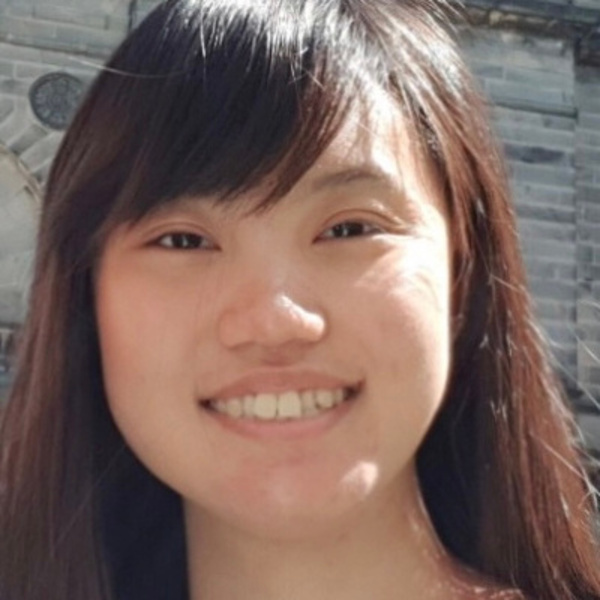
\includegraphics[width=0.06\textheight]{people/dily_ong.jpg}%
        
\includegraphics[width=0.06\textheight]{people/gemini.jpg}%
        
\includegraphics[width=0.06\textheight]{people/harry_bevins.jpg}%
        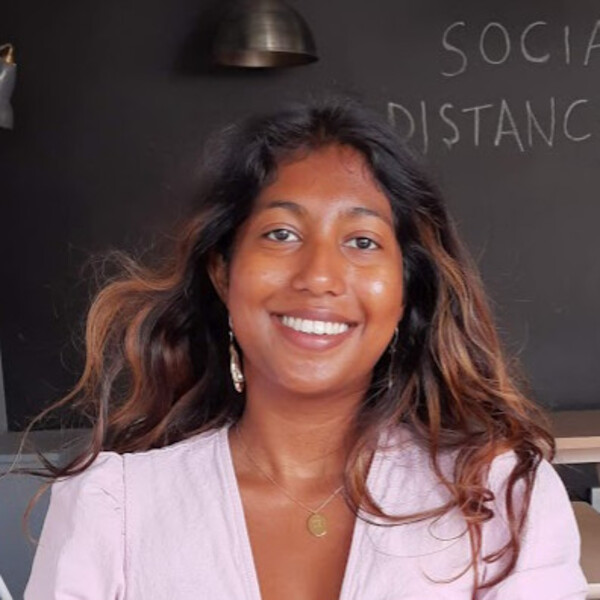
\includegraphics[width=0.06\textheight]{people/metha_prathaban.jpg}%
        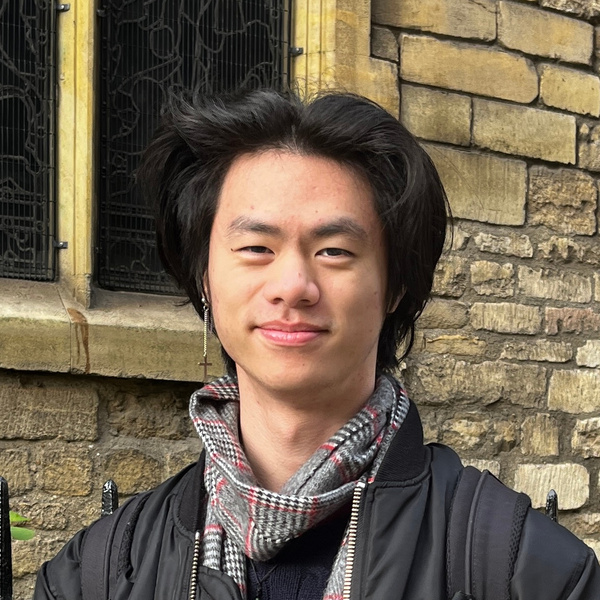
\includegraphics[width=0.06\textheight]{people/ming_yang.jpg}%
        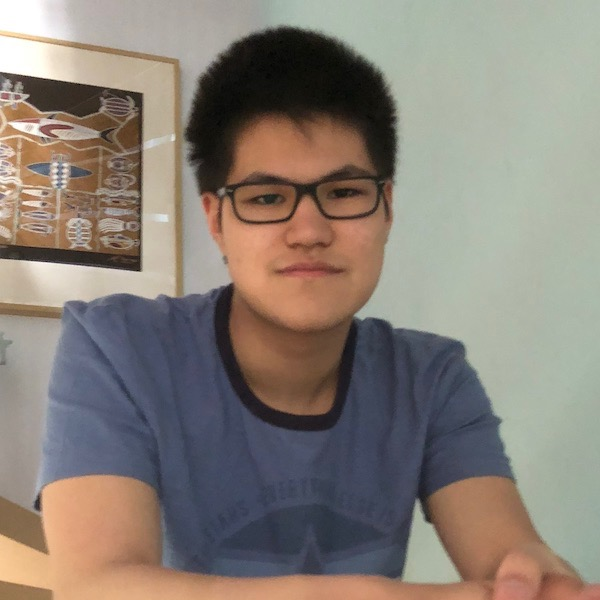
\includegraphics[width=0.06\textheight]{people/namu_kroupa.jpg}%
        
\includegraphics[width=0.06\textheight]{people/openai.jpg}%
        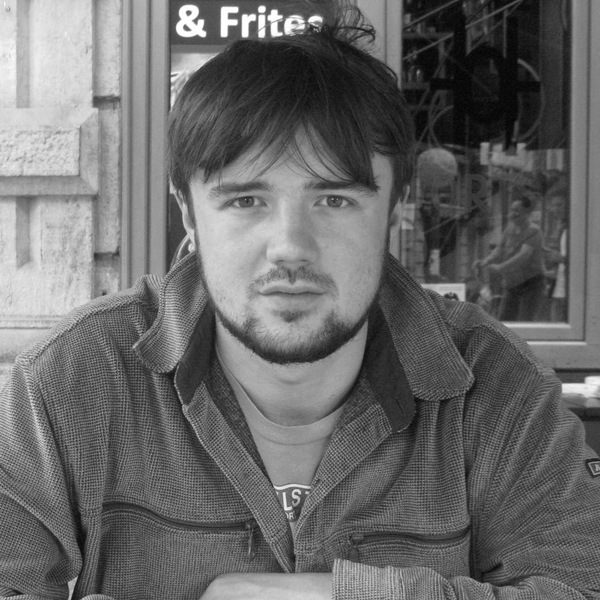
\includegraphics[width=0.06\textheight]{people/sam_leeney.jpg}%
        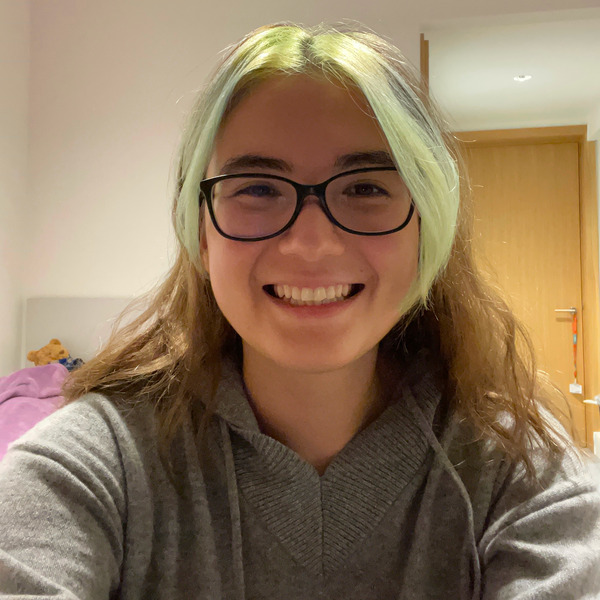
\includegraphics[width=0.06\textheight]{people/sinah_legner.jpg}%
        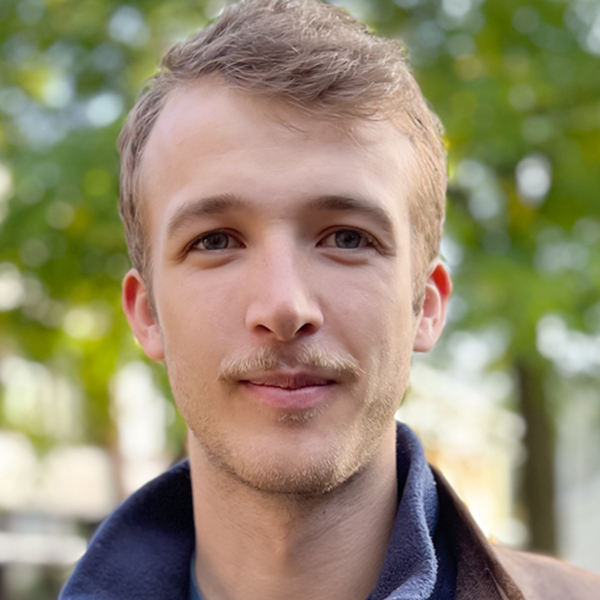
\includegraphics[width=0.06\textheight]{people/toby_lovick.jpg}%
        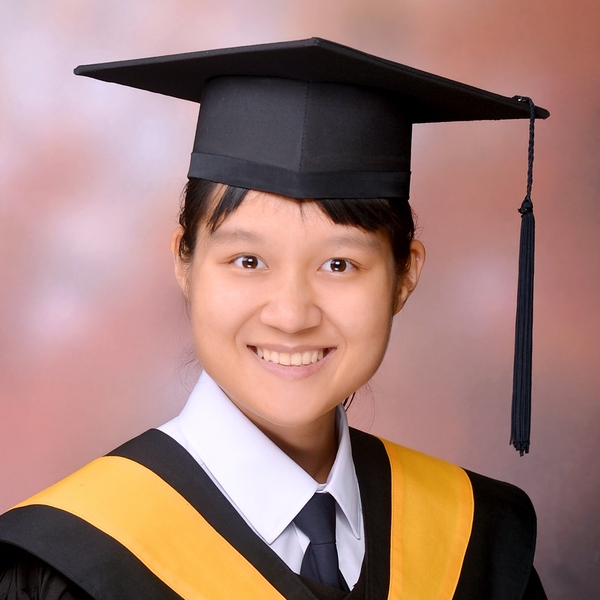
\includegraphics[width=0.06\textheight]{people/wei-ning_deng.jpg}%
        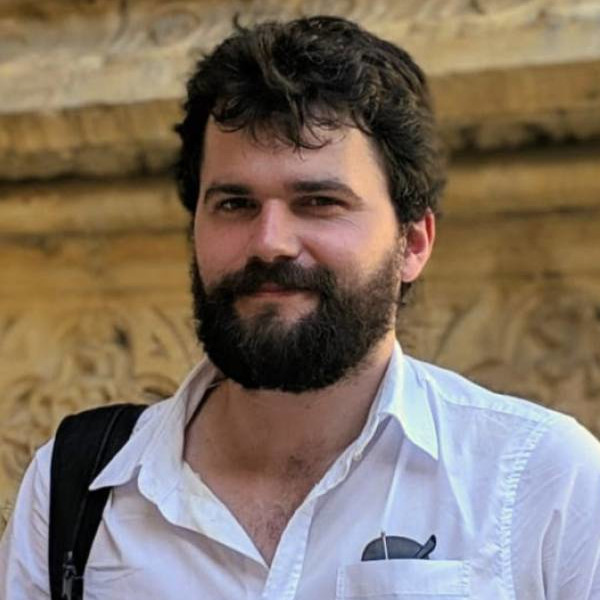
\includegraphics[width=0.06\textheight]{people/will_handley.jpg}%
        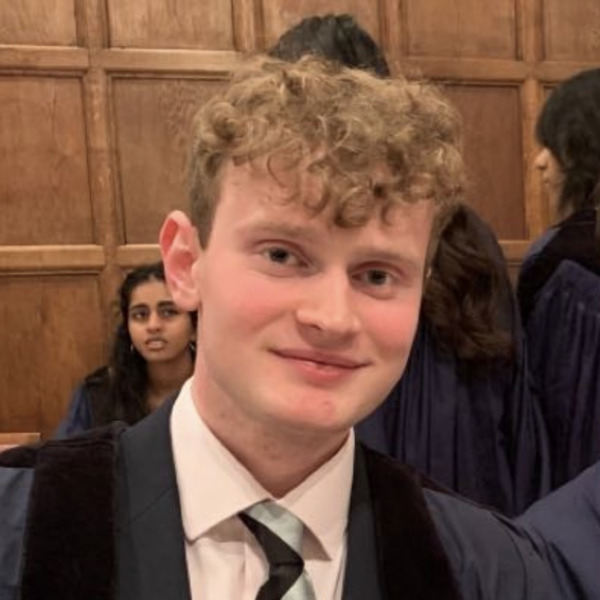
\includegraphics[width=0.06\textheight]{people/will_templeton.jpg}%
    };
\end{frame}

\end{document}
